\documentclass[conference]{IEEEtran}

\usepackage{amsmath,amssymb,amsthm}
\usepackage{booktabs}
\usepackage{graphicx}
\usepackage{cite}
\usepackage{url}
\usepackage{algorithmic}

\graphicspath{{figures/}}
\newcommand{\method}{HSA-CP}
\newtheorem{proposition}{Proposition}
\newtheorem{theorem}{Theorem}
\newtheorem{corollary}{Corollary}
\newcounter{algorithm}
\newcommand{\algcaption}[1]{%
  \refstepcounter{algorithm}\noindent\textbf{Algorithm \thealgorithm: #1}\par\smallskip}

\begin{document}

\title{HSA-CP: Hierarchical Sector-Adaptive Conformal Prediction\\
for Large Cross-Sections of Equity Returns}

\author{\IEEEauthorblockN{Sana Gaied Chortane}
\IEEEauthorblockA{ERIC, Universit\'e Lumi\`ere Lyon 2\\
Lyon, France}}

\maketitle

\begin{abstract}
Forecasting hundreds of financial time series creates an uncertainty-quantification trade-off: asset-wise calibration is noisy, whereas market-wide calibration can hide persistent sector heterogeneity. We introduce Hierarchical Sector-Adaptive Conformal Prediction (\method), an online wrapper combining asset, sector, and market conformal quantiles through sector-specific exponential weights and a feedback controller. Two deterministic results characterize the procedure: a finite-horizon sector calibration identity and a regret bound for the clipped normalized Hedge losses. We evaluate 121,744 one-day-ahead intervals for 501 securities from a fixed S\&P 500 snapshot. The cohort is locked before architecture selection using only January--May 2024 availability; point-model tuning ends in 2023, architecture and online-rate selection use June--December 2024, and 2025 is reserved for final evaluation. At nominal 90\% coverage, \method\ attains 90.0455\% coverage, the lowest mean interval score (0.096016), and the lowest asset-level and cross-sectional 20-day calibration errors among eight primary methods. Sector coverages range from 89.7662\% to 90.4000\%. Without re-tuning, empirical coverages at nominal 80\%, 90\%, and 95\% are 79.9588\%, 90.0455\%, and 95.1883\%. Newey--West tests with Holm correction and moving-block bootstraps support improvements over four baselines; evidence against the remaining methods is weaker. The results support causal hierarchical pooling without claiming exact conditional coverage for dependent returns.
\end{abstract}

\begin{IEEEkeywords}
conformal prediction, online calibration, financial time series, uncertainty quantification, hierarchical data, big data analytics
\end{IEEEkeywords}

\section{Introduction}

Large financial panels combine weak point predictability, distribution shift, and strong cross-sectional dependence. Volatility clusters through time, undermining the exchangeability assumption behind classical conformal prediction (CP) \cite{vovk2005algorithmic,lei2018distribution}. Securities also share market and sector shocks while retaining idiosyncratic dynamics. A useful interval method must therefore update causally, borrow strength across related series, and expose rather than conceal group failures.

The cross-section creates a calibration trade-off. A rolling asset quantile contains relatively few recent scores and can be unstable. A market quantile contains thousands of scores but can average away sector differences. Sector pooling is intermediate, but the best scale may change over time. This motivates a hierarchy of calibration experts rather than one permanently chosen pool.

We propose Hierarchical Sector-Adaptive Conformal Prediction (\method). Given a causal point forecast and lagged volatility scale, the method forms normalized residual scores and three conformal quantiles: asset, sector, and market. Sector-specific exponential weights aggregate their clipped normalized interval losses. A sector feedback state then adjusts the mixture using realized cross-sectional miscoverage. All intervals for date $t$ are issued before any date-$t$ outcome is used. Figure~\ref{fig:architecture} gives the causal workflow.

\begin{figure*}[t]
  \centering
  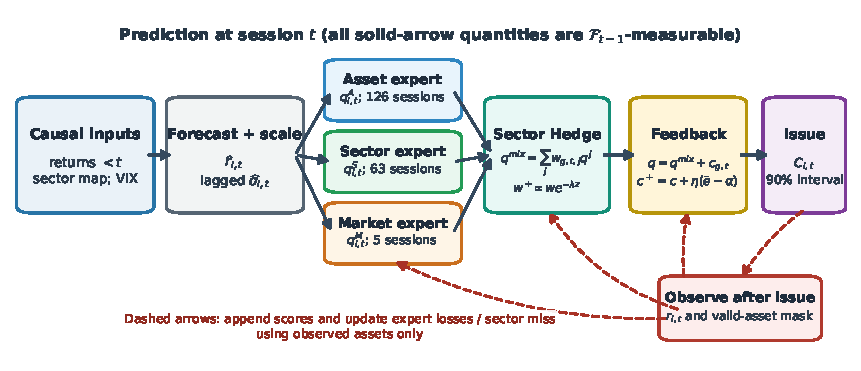
\includegraphics[width=0.98\textwidth]{fig1_hsa_architecture.pdf}
  \caption{Causal \method\ workflow. Solid arrows form the pre-outcome prediction path; dashed arrows update score histories, sector weights, and controller states only after date-$t$ returns are observed.}
  \label{fig:architecture}
\end{figure*}

Our empirical setting contains 503 securities from a May 23, 2024 S\&P 500 constituent snapshot and 1,699 sessions through December 2025. A cohort of 501 securities is locked at May 31, 2024 using only pre-lock return availability. Natural missing values after acquisitions or delistings are retained rather than used as a future-dependent exclusion rule. The 2025 evaluation comprises 121,744 valid asset-days across 11 GICS sectors.

The contributions are fourfold:
\begin{itemize}
 \item a causal hierarchical conformal architecture combining asset, sector, and market score pools;
 \item an exact sector calibration identity, a finite-horizon corollary, and a Hedge regret theorem aligned with the implemented clipped loss;
 \item a corrected anti-leakage benchmark with a pre-validation universe lock, leave-one-out sector features, training-only preprocessing, and validation-only tuning;
 \item an evaluation of eight primary methods using global and local calibration, efficiency, sector and regime robustness, HAC inference, moving-block bootstraps, three nominal levels, scale ablations, and an empirical scalability benchmark.
\end{itemize}
The scope is deliberately limited: our deterministic online results do not imply finite-sample conditional coverage under arbitrary dependent returns.

\section{Related Work}

Classical CP provides distribution-free marginal coverage under exchangeability \cite{vovk2005algorithmic,lei2018distribution}. Weighted CP treats covariate shift when likelihood ratios are known or estimable \cite{tibshirani2019covariate}; non-exchangeable CP quantifies degradation under drift \cite{barber2023beyond}. Financial returns instead display serial dependence, heavy tails, and volatility clustering, so classical guarantees cannot be transferred without their assumptions.

Sequential methods include EnbPI's rolling ensemble residuals \cite{xu2021enbpi}, SPCI's conditional score-quantile forecasts \cite{xu2023spci}, Adaptive Conformal Inference (ACI) \cite{gibbs2021adaptive}, AgACI's aggregation of learning rates \cite{zaffran2022adaptive}, strongly adaptive online CP \cite{bhatnagar2023saocp}, and conformal inference under arbitrary shifts \cite{gibbs2024arbitrary}. Conformal PID interprets online threshold adaptation through feedback control \cite{angelopoulos2023pid}. Our controller is closest to proportional quantile tracking, while our distinct component is the asset--sector--market hierarchy with one weight vector and one controller state per sector.

Marginal coverage can hide systematic group failures. Multivalid prediction targets coverage across user-defined groups in adversarial sequences \cite{bastani2022mvp}; batch multivalid and Kandinsky CP broaden group-aware events \cite{jung2022batch,bairaktari2025kandinsky}. Recent parameter-free group-conditional online CP pursues stronger worst-case group targets \cite{bharti2026group}. In contrast, \method\ is domain-specialized: disjoint sectors are feedback groups, and hierarchical pooling targets empirical efficiency. We do not claim parameter-free or multivalid guarantees. Financial applications remain limited and include market-return control experiments and conformal stock-selection sets \cite{angelopoulos2023pid,kaya2025stocks}.

\begin{table*}[t]
\centering
\caption{Positioning relative to representative CP families; guarantees require each cited work's assumptions.}
\label{tab:positioning}
\scriptsize
\setlength{\tabcolsep}{2.5pt}
\begin{tabular}{p{0.13\textwidth}p{0.20\textwidth}p{0.18\textwidth}p{0.16\textwidth}p{0.23\textwidth}}
\toprule
Family & Adaptation & Cross-series structure & Group target & Guarantee or objective\\
\midrule
Split CP \cite{lei2018distribution} & Fixed calibration quantile & None & None & Finite-sample marginal under exchangeability\\
EnbPI/SPCI \cite{xu2021enbpi,xu2023spci} & Rolling or conditional score model & Temporal score history & None & Coverage under stated dependence/consistency conditions\\
ACI/AgACI \cite{gibbs2021adaptive,zaffran2022adaptive} & Error-level update/rate experts & Temporal experts & None & Long-run calibration and adaptive efficiency\\
SAOCP/FACI \cite{bhatnagar2023saocp,gibbs2024arbitrary} & Local-regret online learning & Temporal interval experts & None & Strong/local adaptive regret and coverage\\
Conformal PID \cite{angelopoulos2023pid} & Feedback and scorecasting & Optional external series & None & Deterministic long-run calibration conditions\\
MVP/group OCP \cite{bastani2022mvp,bharti2026group} & Multivalid/group updates & User groups & Explicit groups & Adversarial empirical/group-conditional targets\\
\method\ (ours) & Sector Hedge and feedback & Asset--sector--market & Fixed sectors & Identity, Hedge regret, and empirical panel study\\
\bottomrule
\end{tabular}
\end{table*}

\section{Problem Formulation}

Let $i\in\{1,\ldots,N\}$ index assets, $t$ sessions, and $g(i)\in\{1,\ldots,G\}$ the sector of asset $i$. At the beginning of $t$, a forecaster uses $\mathcal F_{t-1}$ to issue $\widehat r_{i,t}$ for log return $r_{i,t}$ and a symmetric interval
\begin{equation}
 C_{i,t}=[\widehat r_{i,t}-h_{i,t},\widehat r_{i,t}+h_{i,t}],
\end{equation}
where $h_{i,t}$ is $\mathcal F_{t-1}$-measurable. The target error is $\alpha=0.10$. Scores are normalized by a lagged volatility estimate $\widehat\sigma_{i,t}>0$:
\begin{equation}
 s_{i,t}=\frac{|r_{i,t}-\widehat r_{i,t}|}{\widehat\sigma_{i,t}}.
 \label{eq:score}
\end{equation}
We use a 21-session exponentially weighted standard deviation, shifted one day and floored by a constant estimated on training data only.

For $l\leq u$, the interval score is \cite{gneiting2007scoring}
\begin{equation}
 \mathrm{IS}_{\alpha}(r,l,u)=(u-l)+\frac{2}{\alpha}(l-r)_{+}
 +\frac{2}{\alpha}(r-u)_{+}.
 \label{eq:is}
\end{equation}
We also report coverage, absolute coverage gap, width, the 10th percentile of asset coverage, and worst sector/regime coverage. Let $\widehat c_{i,t}^{(20)}$ be rolling 20-day asset coverage and $\widehat c_{t}^{X,(20)}$ rolling 20-day coverage of the daily cross-sectional mean. Define
\begin{align}
 \mathrm{ALCE20}&=\operatorname{mean}_{i,t}|\widehat c_{i,t}^{(20)}-(1-\alpha)|,\\
 \mathrm{XLCE20}&=\operatorname{mean}_{t}|\widehat c_{t}^{X,(20)}-(1-\alpha)|.
\end{align}
This separates asset instability from market-wide temporal drift.

\section{Hierarchical Sector-Adaptive CP}

\subsection{Hierarchical Experts}

For a finite multiset $S$ of $m$ scores, define the exact conformal order statistic
\begin{equation}
 Q_{1-\alpha}(S)=S_{(k)},\quad
 k=\min\{m,\max(1,\lceil(m+1)(1-\alpha)\rceil)\}.
 \label{eq:cquantile}
\end{equation}
Direct indexing avoids software-dependent interpolation and off-by-one errors. At date $t$, the three experts are
\begin{align}
 q^A_{i,t}&=Q_{1-\alpha}\{s_{i,\tau}:t-126\leq\tau<t\},\\
 q^S_{i,t}&=Q_{1-\alpha}\{s_{j,\tau}:g(j)=g(i),t-63\leq\tau<t\},\\
 q^M_{i,t}&=Q_{1-\alpha}\{s_{j,\tau}:1\leq j\leq N,t-5\leq\tau<t\}.
\end{align}
Missing scores are omitted. The windows balance idiosyncratic persistence, sector pooling, and rapid market response.

\subsection{Sector Hedge Aggregation}

For $J=3$, sector $g$ has weights $\mathbf w_{g,t}$, initialized uniformly. Its mixed threshold is
\begin{equation}
 q^{\rm mix}_{i,t}=\sum_{j\in\{A,S,M\}}w_{g(i),t,j}q^j_{i,t}.
 \label{eq:mixture}
\end{equation}
After observing $t$, expert $j$ receives the scale-free symmetric-interval loss
\begin{equation}
 L_{g,t,j}=\frac{1}{|I_{g,t}|}\sum_{i\in I_{g,t}}
 \left[2q^j_{i,t}+\frac{2}{\alpha}(s_{i,t}-q^j_{i,t})_+\right],
\end{equation}
where $I_{g,t}$ contains observed sector assets. With $a_{g,t}=\max\{\operatorname{median}_jL_{g,t,j},10^{-6}\}$, define $z_{g,t,j}=\min\{10,L_{g,t,j}/a_{g,t}\}\in[0,B]$, $B=10$, and update
\begin{equation}
 w_{g,t+1,j}=\frac{w_{g,t,j}e^{-\lambda z_{g,t,j}}}
 {\sum_{k=1}^{J}w_{g,t,k}e^{-\lambda z_{g,t,k}}},\quad \lambda=0.04.
 \label{eq:hedge}
\end{equation}

\begin{theorem}[Hedge regret for the implemented loss]
For any sequence $\mathbf z_{g,t}\in[0,B]^J$ and uniform initial weights, update \eqref{eq:hedge} satisfies
\begin{equation}
 \sum_{t=1}^{T}\langle\mathbf w_{g,t},\mathbf z_{g,t}\rangle-
 \min_j\sum_{t=1}^{T}z_{g,t,j}
 \leq \frac{\log J}{\lambda}+\frac{\lambda B^2T}{8}.
 \label{eq:hedgeregret}
\end{equation}
\end{theorem}
\begin{proof}
Let $W_t=\sum_j\exp[-\lambda\sum_{\tau<t}z_{g,\tau,j}]$. Hoeffding's lemma for $z\in[0,B]$ gives $\log(W_{t+1}/W_t)\leq-\lambda\langle\mathbf w_{g,t},\mathbf z_{g,t}\rangle+\lambda^2B^2/8$. Summing and using $\log(W_{T+1}/W_1)\geq-\lambda\min_j\sum_tz_{g,t,j}-\log J$ yields \eqref{eq:hedgeregret}.
\end{proof}
The theorem applies exactly to the normalized clipped expert loss $z$, not to the unbounded raw return interval score.

\subsection{Sector Feedback and Finite-Horizon Calibration}

Sector $g$ maintains state $c_{g,t}$, initialized at zero. The issued threshold and half-width are
\begin{equation}
 q^{\method}_{i,t}=\max\{0,q^{\rm mix}_{i,t}+c_{g(i),t}\},\quad
 h_{i,t}=q^{\method}_{i,t}\widehat\sigma_{i,t}.
 \label{eq:finalq}
\end{equation}
After outcomes arrive, let
\begin{equation}
 \bar e_{g,t}=\frac{1}{|I_{g,t}|}\sum_{i\in I_{g,t}}
 \mathbb 1\{s_{i,t}>q^{\method}_{i,t}\}.
\end{equation}
The validation-selected feedback rate is $\eta=0.05$:
\begin{equation}
 c_{g,t+1}=c_{g,t}+\eta(\bar e_{g,t}-\alpha).
 \label{eq:controller}
\end{equation}

\begin{proposition}[Exact sector calibration identity]
For any score sequence and any $T$ sessions on which sector $g$ is updated,
\begin{equation}
 \frac1T\sum_{t=1}^{T}\bar e_{g,t}-\alpha
 =\frac{c_{g,T+1}-c_{g,1}}{\eta T}.
 \label{eq:identity}
\end{equation}
\end{proposition}
\begin{proof}
Rearrange \eqref{eq:controller}, sum over $t$, and telescope the controller increments.
\end{proof}

\begin{corollary}[Finite-horizon deviation]
If $|c_{g,T+1}-c_{g,1}|\leq D_g$, then
\begin{equation}
 \left|\frac1T\sum_{t=1}^{T}\bar e_{g,t}-\alpha\right|
 \leq\frac{D_g}{\eta T}.
\end{equation}
Hence sublinear controller excursion implies asymptotic sector-average calibration.
\end{corollary}
\begin{proof}
Take absolute values in \eqref{eq:identity} and apply the assumed bound.
\end{proof}
This result is deterministic, but it does not bound $D_g$ for every unbounded financial score sequence and does not establish asset-wise conditional coverage. In the 2025 evaluation, the recomputed left- and right-hand sides agree within $2.1\times10^{-17}$ for every sector.

\begin{figure*}[t]
\small
\hrule\vspace{3pt}
\algcaption{HSA-CP Online Prediction and Update}\label{alg:hsa}
\begin{algorithmic}[1]
\REQUIRE Target error $\alpha$; windows $(W_A,W_S,W_M)=(126,63,5)$; Hedge rate $\lambda=.04$; controller rate $\eta=.05$
\STATE Initialize $w_{g,1,j}=1/3$ for $j\in\{A,S,M\}$, $c_{g,1}=0$, and causal score histories using pre-date-$t$ observations.
\FOR{trading sessions $t$ in chronological order}
  \STATE Using $\mathcal F_{t-1}$, compute $\widehat r_{i,t}$ and lagged $\widehat\sigma_{i,t}$ for every asset.
  \STATE Compute $q^A_{i,t}$, $q^S_{i,t}$, and $q^M_{i,t}$ from histories ending at $t-1$ with windows $W_A,W_S,W_M$.
  \FOR{sectors $g$}
    \STATE Normalize $\mathbf w_{g,t}$; set $q^{\rm mix}_{i,t}=\sum_jw_{g,t,j}q^j_{i,t}$ and $q_{i,t}=\max\{0,q^{\rm mix}_{i,t}+c_{g,t}\}$.
  \ENDFOR
  \STATE Issue the complete cross-section $C_{i,t}=[\widehat r_{i,t}-\widehat\sigma_{i,t}q_{i,t},\widehat r_{i,t}+\widehat\sigma_{i,t}q_{i,t}]$ before observing any $r_{i,t}$.
  \STATE Observe date-$t$ returns and define $I_{g,t}$ as the assets in sector $g$ with observed return, forecast, and scale.
  \FOR{sectors $g$ with $|I_{g,t}|>0$}
    \STATE Compute $s_{i,t}$ for $i\in I_{g,t}$, expert losses $L_{g,t,j}$, and clipped normalized losses $z_{g,t,j}\in[0,10]$.
    \STATE Update $w_{g,t+1,j}\propto w_{g,t,j}\exp(-\lambda z_{g,t,j})$.
    \STATE Compute $\bar e_{g,t}=|I_{g,t}|^{-1}\sum_{i\in I_{g,t}}\mathbb 1\{s_{i,t}>q_{i,t}\}$ and update $c_{g,t+1}=c_{g,t}+\eta(\bar e_{g,t}-\alpha)$.
  \ENDFOR
  \STATE Append only available scores to their causal histories; leave sectors with $|I_{g,t}|=0$ unchanged.
\ENDFOR
\end{algorithmic}
\vspace{2pt}\hrule
\end{figure*}

Algorithm~\ref{alg:hsa} makes the predict--observe--update order and missing-data mask explicit. After window quantiles are obtained, aggregation and feedback cost $O(NJ+GJ)$ per session, with $J=3$ and $G=11$. The calibration layer never refits the point model.

\section{Experimental Design}

\subsection{Data, Cohort Lock, and Chronology}

Adjusted daily closes span April 1, 2019--December 31, 2025 for a 503-security S\&P 500 snapshot dated May 23, 2024. Provider ticker changes and class-share punctuation are documented. Individual prices are neither interpolated nor forward/backward filled. We compute log returns and retain 501 securities with at least 99\% observed returns from January 1--May 31, 2024. GEV and SOLV lack sufficient pre-lock history and are excluded; no 2025 quotation, acquisition, or delisting field affects selection. Fourteen securities wrongly removed by a future-balanced rule are therefore reinstated. Their natural post-lock missing values remain missing and reduce valid asset-days rather than changing the cohort.

The split dates follow the forecasting chronology rather than a favorable-result search. After the Ridge penalty is selected on calendar 2023, the point forecaster is refit through December 29, 2023. January 2, 2024 is therefore the first subsequent trading session and yields residuals out of sample with respect to the final point-model fit. The initial conformal block ends on May 31, the last session before architecture validation begins on June 3. This gives 105 initial-calibration/burn-in sessions, 147 disjoint validation sessions, and 250 final-evaluation sessions. Using all of 2024 for calibration would leave no independent period for selecting rates and experts; selecting them on 2025 would leak test outcomes. The May 23 date identifies the constituent snapshot, whereas May 31 is the pre-validation availability lock. No 2025 outcome enters either operation.

The static snapshot permits a stable hierarchy but induces historical-selection and survivorship bias. It is a fixed-snapshot forecasting panel, not a point-in-time tradable-index backtest. Causal market regimes compare VIX$(t-1)$ with rolling terciles of earlier lagged VIX values. Table~\ref{tab:data} summarizes the corrected panel, and Algorithm~\ref{alg:protocol} formalizes the leakage controls.

\begin{table}[t]
\centering
\caption{Corrected panel and chronology.}
\label{tab:data}
\small
\begin{tabular}{lr}
\toprule
Quantity & Value\\
\midrule
Snapshot / pre-lock cohort & 503 / 501\\
GICS sectors / full sessions & 11 / 1,699\\
Point-tuning train & 2019-04-01--2022-12-30\\
Point-tuning validation & 2023-01-03--2023-12-29\\
Initial calibration/burn-in (105) & 2024-01-02--2024-05-31\\
Architecture/rate validation (147) & 2024-06-03--2024-12-31\\
Final evaluation (250) & 2025-01-02--2025-12-31\\
Valid final-evaluation intervals & 121,744\\
\bottomrule
\end{tabular}
\end{table}

\begin{figure*}[t]
\small
\hrule\vspace{3pt}
\algcaption{Leakage-Controlled Model Selection and Evaluation}\label{alg:protocol}
\begin{algorithmic}[1]
\REQUIRE Raw adjusted closes, May 23, 2024 snapshot metadata, sectors, and causal market covariates
\STATE Correct provider symbols; compute log returns without price imputation; document the fixed-snapshot interpretation.
\STATE Before architecture validation, lock the cohort at May 31, 2024 using the 99\% January--May availability rule only.
\STATE On the locked cohort, fit each Ridge candidate on 2019--2022 and select its penalty by 2023 MAE.
\STATE Refit the selected Ridge through December 29, 2023 using training-only standardization and volatility-floor estimation.
\STATE Initialize conformal score histories and online states on January 2--May 31, 2024.
\STATE Select baseline rates, the expert set, Hedge rate, and controller rate using June 3--December 31, 2024 only.
\STATE Freeze the point model, cohort, features, windows, architecture, rates, metrics, and inference plan.
\STATE Retain the causally updated state through December 31, 2024; evaluate every valid 2025 asset-day without re-selection.
\STATE Compare daily paired scores using Newey--West HAC tests, Holm correction, and moving-block bootstraps with blocks 5, 10, and 20.
\ENSURE No 2025 outcome is used for cohort construction, point fitting, calibration design, or hyperparameter selection.
\end{algorithmic}
\vspace{2pt}\hrule
\end{figure*}

\subsection{Common Point Forecaster}

All interval methods wrap the same pooled ridge regression \cite{hoerl1970ridge}. Features available by $t-1$ include asset lags 1, 2, and 5; lagged 5- and 21-day means and standard deviations; lagged market return; a leave-one-out equal-weight sector return; lagged VIX and market volatility; causal regime indicators; and sector indicators. The leave-one-out construction avoids mechanically reusing an asset return in its own sector feature. Standardization and the volatility floor use training data only.

The ridge penalty is selected from $\{1,10,25,100\}$ using calendar 2023 only; $100$ is selected and the model is refit through 2023. It uses 583,981 training rows. On 121,744 valid 2025 asset-days, MAE is 0.014070, RMSE 0.021822, sign accuracy 0.510079, and out-of-sample $R^2$ 0.001892. The deliberately modest predictor isolates calibration effects.

\subsection{Baselines and Validation Rules}

We compare SplitCP, 126-day RollingCP, ACI \cite{gibbs2021adaptive}, asset-level proportional control (PControl) \cite{angelopoulos2023pid}, 63-day SectorCP, GraphCP using five training-period correlation neighbors, RegimeCP using causal VIX states, and \method. ACI's rate is selected from $\{.001,.0025,.005,.01,.02\}$ and PControl's from $\{.01,.025,.05,.10,.20\}$ using June--December 2024 only; selected values are .005 and .05. \method's controller and Hedge rates are .05 and .04, also chosen without 2025 outcomes.

The controller is a constitutive component tied to Proposition~1, so controller-free mixtures are diagnostic ablations rather than architecture candidates. Among controller-preserving variants with validation coverage gap at most .005, interval score selects asset--sector--market \method. Graph and regime experts are rejected before final evaluation.

\subsection{Inference}

For each comparator, we average interval score across observed assets by date and analyze the paired daily difference, comparator minus \method. A one-sided mean test uses a Newey--West heteroskedasticity-and-autocorrelation-consistent standard error with lag 10 \cite{newey1987simple}; seven $p$-values receive Holm correction \cite{holm1979}. Moving-block bootstrap (MBB) 95\% intervals use 2,000 replicates and block lengths 5, 10, and 20 \cite{kunsch1989bootstrap}. We call an improvement robust only if all three lower bounds exceed zero.

\section{Results}

\subsection{Overall Calibration and Efficiency}

Table~\ref{tab:main} reports the corrected 2025 evaluation. \method\ reaches 0.900455 coverage, a 0.000455 gap from target, and the lowest interval score, ALCE20, and XLCE20 among the eight primary methods. Score reductions range from 1.10\% versus SectorCP to 2.43\% versus RegimeCP. ACI has a slightly smaller marginal coverage gap, but larger local errors and score. The result is therefore not merely wider intervals achieving nominal coverage.

\begin{table*}[t]
\centering
\caption{Final 2025 results on 121,744 valid intervals. Gap is $|\mathrm{coverage}-.90|$; lower score, ALCE20, and XLCE20 are better.}
\label{tab:main}
\small
\setlength{\tabcolsep}{4.6pt}
\begin{tabular}{lrrrrrrrr}
\toprule
Method & Coverage & Gap & Mean width & Median width & Score & ALCE20 & XLCE20 & Worst sector\\
\midrule
SplitCP   & .910739 & .010739 & .067636 & .057775 & .097656 & .050731 & .022566 & .904000\\
RollingCP & .904940 & .004940 & .066810 & .056737 & .097991 & .049374 & .023006 & .901968\\
ACI       & .899708 & \textbf{.000292} & .066097 & .055770 & .098324 & .049864 & .023523 & .897298\\
PControl  & .903223 & .003223 & .065511 & .055894 & .097160 & .048231 & .022243 & .900000\\
SectorCP  & .898057 & .001943 & \textbf{.064795} & .054744 & .097088 & .051046 & .024715 & .894078\\
GraphCP   & .899116 & .000884 & .065955 & .055424 & .097790 & .050896 & .024879 & .894105\\
RegimeCP  & .903240 & .003240 & .066897 & .056774 & .098412 & .048905 & .020391 & .897994\\
\method   & .900455 & .000455 & .065386 & \textbf{.054555} & \textbf{.096016} & \textbf{.047270} & \textbf{.017636} & .897662\\
\bottomrule
\end{tabular}
\end{table*}

\begin{figure*}[t]
  \centering
  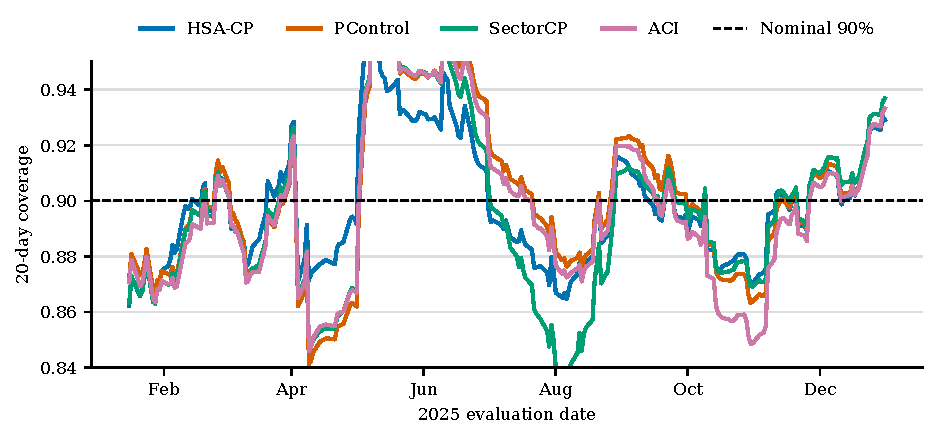
\includegraphics[width=0.94\textwidth]{fig2_rolling_coverage.pdf}
  \caption{Twenty-day rolling cross-sectional coverage in 2025. \method\ has the lowest XLCE20, but common shifts remain visible.}
  \label{fig:rolling}
\end{figure*}

\subsection{Dependence-Robust Comparisons}

Table~\ref{tab:stats} separates HAC significance from block-length robustness. RegimeCP, ACI, RollingCP, and GraphCP have positive MBB lower bounds for all three block lengths and Holm-adjusted HAC $p<.05$. SplitCP passes the HAC test and 10/20-day bootstraps, but its 5-day lower bound is slightly negative. PControl and SectorCP are not significant after Holm correction and have negative lower bounds. The supported claim is therefore improvement over four, not all seven, comparators.

\begin{table*}[t]
\centering
\caption{Daily score difference, comparator minus \method. $L_b$ is the MBB 95\% lower bound at block length $b$.}
\label{tab:stats}
\small
\setlength{\tabcolsep}{7.5pt}
\begin{tabular}{lrrrrrc}
\toprule
Comparator & Mean diff. & Holm HAC $p$ & $L_5$ & $L_{10}$ & $L_{20}$ & Robust all $b$\\
\midrule
RegimeCP  & .002396 & .0124 & .000718 & .000933 & .001046 & Yes\\
ACI       & .002308 & .0124 & .000717 & .000985 & .001015 & Yes\\
RollingCP & .001974 & .0279 & .000290 & .000616 & .000717 & Yes\\
GraphCP   & .001774 & .0437 & .000365 & .000453 & .000371 & Yes\\
SplitCP   & .001640 & .0491 & $-.000231$ & .000235 & .000477 & No\\
PControl  & .001144 & .1474 & $-.000695$ & $-.000224$ & $-.000013$ & No\\
SectorCP  & .001072 & .1474 & $-.000478$ & $-.000162$ & $-.000160$ & No\\
\bottomrule
\end{tabular}
\end{table*}

\subsection{Sector, Regime, and Online Behavior}

All sector coverages lie between .897662 and .904000 (Table~\ref{tab:sectors}). Across causal VIX regimes, \method\ covers .912331 on 59 low-volatility days, .892895 on 95 normal days, and .900637 on 96 high days; widths rise from .054772 to .077892. The normal-regime shortfall and asset-coverage 10th percentile of .8864 show that sector feedback is not per-asset or regime-conditional calibration.

\begin{table}[t]
\centering
\caption{Final \method\ results by sector.}
\label{tab:sectors}
\scriptsize
\setlength{\tabcolsep}{3.0pt}
\begin{tabular}{lrrrr}
\toprule
Sector & $N$ & Coverage & Width & Score\\
\midrule
Communication Services & 22 & .904000 & .065264 & .095416\\
Consumer Discretionary & 52 & .901462 & .073708 & .107728\\
Consumer Staples & 38 & .901667 & .057008 & .082351\\
Energy & 22 & .902526 & .071391 & .099067\\
Financials & 71 & .898805 & .055013 & .080280\\
Health Care & 63 & .902164 & .069360 & .104940\\
Industrials & 78 & .897662 & .061224 & .091153\\
Information Technology & 65 & .899238 & .083511 & .125114\\
Materials & 28 & .902074 & .072017 & .106020\\
Real Estate & 31 & .901935 & .051936 & .072883\\
Utilities & 31 & .900516 & .053998 & .075597\\
\bottomrule
\end{tabular}
\end{table}

\begin{figure*}[t]
  \centering
  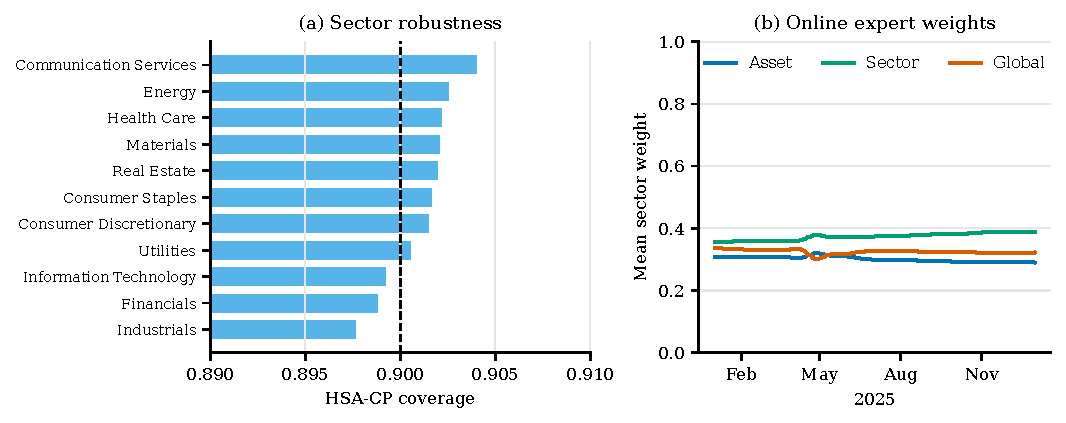
\includegraphics[width=0.94\textwidth]{fig3_sector_and_weights.pdf}
  \caption{(a) Final sector coverages. (b) Ten-day smoothed expert weights averaged across sectors.}
  \label{fig:robustness}
\end{figure*}

Mean 2025 weights are .301 asset, .375 sector, and .324 market. They remain mixed, although the benefit of learned weights is modest. Equal weights score .084514 versus .084512 on validation and .095954 versus .096016 in final evaluation. Hedge therefore supplies an online no-regret mechanism but not a material empirical advantage in this sample.

\subsection{Ablations and Sensitivity}

Table~\ref{tab:ablation} records validation rather than test-driven choices. Controller-free aggregation has a lower validation score (.084430) and remains within the .005 coverage tolerance, but it is excluded from architecture selection because feedback and Proposition~1 define the proposed method. This is a calibration--efficiency trade-off, not evidence that every component improves interval score. Among controller-preserving variants, \method\ has the best eligible validation score. Graph and regime additions worsen it.

\begin{table}[t]
\centering
\caption{Architecture validation, June--December 2024.}
\label{tab:ablation}
\scriptsize
\setlength{\tabcolsep}{3.0pt}
\begin{tabular}{lrrrr}
\toprule
Variant & Coverage & Gap & Width & Score\\
\midrule
No controller (diagnostic) & .904399 & .004399 & .057854 & \textbf{.084430}\\
\method\ (selected) & .903700 & .003700 & .057840 & .084512\\
Equal weights & .903798 & .003798 & .057875 & .084514\\
Add graph expert & .904119 & .004119 & .057823 & .084565\\
No sector expert & .903589 & .003589 & .058092 & .084699\\
Sector controller only & .903253 & .003253 & .057594 & .084712\\
No global expert & .903924 & .003924 & .057850 & .084807\\
Add regime expert & .904050 & .004050 & .058169 & .084810\\
Asset controller only & .904985 & .004985 & .058507 & .085218\\
\bottomrule
\end{tabular}
\end{table}

Validation-only controller rates from .05 to .25 yield coverage .903700--.902820 and scores .084512--.084884; .05 is selected. Hedge rates .01--.16 change score by less than $2\times10^{-6}$ around .084513. No rate is retuned on 2025. In final-evaluation diagnostics, removing the controller scores .095923 but covers .902747; this post-selection ablation is reported without redesigning the method.

\subsection{Nominal Levels, Scale, and Scalability}

Table~\ref{tab:extended} applies the frozen architecture to two additional nominal levels and two scale ablations. Coverage gaps remain below .002 at 80\%, 90\%, and 95\% without re-tuning. The primary lagged EWM scale has the best interval score and asset-local calibration among the three scale choices. Removing volatility normalization slightly reduces width but degrades interval score and ALCE20, consistent with volatility normalization being useful for heterogeneous assets.

The cohort result is also insensitive to the questioned May cutoff under the primary availability rule. Cutoffs April 30, May 23, and May 31 combined with thresholds 98\% or 99\% all select the same 501 securities (Jaccard similarity 1.0). A strict 100\% rule at May 31 removes 14 securities because of isolated late-May missing returns; this motivates the pre-specified 99\% tolerance rather than claiming May 31 is an optimal date.

The reference Python calibration layer processes the full 501-asset cross-section in 2.725 ms per session (median over five repeats of 60 sessions), versus .917 ms for 50 assets. The empirical log--log slope is .469 because fixed sector overhead and vectorized pooling dominate at small $N$; this is a machine-specific implementation benchmark, not an asymptotic complexity claim. The algorithmic aggregation/update cost after quantile construction remains $O(NJ+GJ)$.

\begin{table*}[t]
\centering
\caption{Additional frozen-configuration checks. Panels A--B evaluate the same 121,744 valid 2025 intervals; no rate, window, or architecture is re-selected. Panel C is a single-core reference benchmark; lower time is better.}
\label{tab:extended}
\scriptsize
\setlength{\tabcolsep}{4.2pt}
\begin{tabular}{llrrrrrr}
\toprule
Panel & Configuration & Coverage & Gap & Mean width & Score & ALCE20 & XLCE20\\
\midrule
A: nominal level & 80\% & .799588 & .000412 & .046479 & .073322 & .069107 & .026067\\
 & 90\% (primary) & .900455 & .000455 & .065386 & .096016 & .047270 & .017636\\
 & 95\% & .951883 & .001883 & .086959 & .123592 & .030956 & .011231\\
\midrule
B: scale at 90\% & Lagged EWM21 (primary) & .900455 & .000455 & .065386 & .096016 & .047270 & .017636\\
 & Lagged rolling-21 & .901145 & .001145 & .066764 & .097620 & .049253 & .016507\\
 & No volatility normalization & .899437 & .000563 & .065035 & .096813 & .053141 & .008987\\
\midrule
\multicolumn{2}{l}{C: assets $N$} & \multicolumn{2}{c}{Median ms/session} & \multicolumn{2}{c}{Intervals/second} & \multicolumn{2}{c}{Runtime vs. $N=50$}\\
\cmidrule(lr){3-4}\cmidrule(lr){5-6}\cmidrule(lr){7-8}
\multicolumn{2}{l}{50}  & \multicolumn{2}{c}{.917} & \multicolumn{2}{c}{54,536}  & \multicolumn{2}{c}{1.000}\\
\multicolumn{2}{l}{100} & \multicolumn{2}{c}{1.130} & \multicolumn{2}{c}{88,505}  & \multicolumn{2}{c}{1.232}\\
\multicolumn{2}{l}{250} & \multicolumn{2}{c}{1.705} & \multicolumn{2}{c}{146,649} & \multicolumn{2}{c}{1.859}\\
\multicolumn{2}{l}{501} & \multicolumn{2}{c}{2.725} & \multicolumn{2}{c}{183,851} & \multicolumn{2}{c}{2.972}\\
\bottomrule
\end{tabular}
\end{table*}

\section{Discussion and Limitations}

The experiment shows that a large cross-section can stabilize uncertainty estimates even when point predictability is weak. The short market expert reacts quickly, the sector expert captures persistent group structure, and the asset expert preserves idiosyncrasy. Sector feedback makes the average error mechanically auditable through Proposition~1. Validation also supplies negative evidence: correlation-neighbor and regime experts do not improve the selected architecture.

The effect must be stated conservatively. \method\ has the best primary-method score and local calibration metrics, but block-length-robust evidence holds for four comparators. Controller-free and equal-weight ablations are competitive; the contribution is therefore the auditable hierarchical control framework rather than universal domination.

The fixed 2024 snapshot creates historical-selection and survivorship bias. Future studies should use point-in-time membership and institutional corporate-action identifiers. Public adjusted-close data can be revised by vendors. The 2025 period has only 250 sessions, and one validation year cannot represent every market state. Multiple rolling-origin years, other markets, and longer horizons are necessary.

The theory is also limited. The controller identity does not bound its own state for arbitrary unbounded scores; the Hedge theorem concerns normalized clipped expert loss. Neither provides finite-sample conditional coverage for dependent returns. Fixed disjoint sectors do not ensure asset-, regime-, or intersectional-group coverage. Parameter-free group-conditional online CP is an important future comparator \cite{bharti2026group}.

The reproducibility package records the snapshot and mappings, corrected cohort rule, partitions, tuning grids, features, daily results, online paths, controller-identity diagnostics, figures, and table scripts. The only stochastic calculation is the MBB with recorded seeds. Raw/derived market-data redistribution remains subject to provider terms. The intervals are research outputs, not an investment strategy.

\section{Conclusion}

We presented \method, a causal online conformal wrapper for a large panel of equity returns. It combines asset, sector, and market quantiles, tracks clipped expert losses, and corrects sector-average errors through feedback. The corrected experiment locks 501 securities before validation and evaluates 121,744 intervals in 2025. \method\ achieves 90.0455\% coverage, the lowest primary-method interval score, ALCE20, and XLCE20, and sector coverage from 89.7662\% to 90.4000\%. Dependence-aware inference supports robust improvements over four baselines while revealing weaker evidence against the closest methods. Hierarchical pooling is a practical middle ground between noisy asset calibration and overly broad market pooling, provided both its empirical gains and theoretical limits are reported transparently.

\IfFileExists{IEEEtran.bst}{\bibliographystyle{IEEEtran}}{\bibliographystyle{ieeetr}}
\bibliography{references}

\end{document}
